%%%%%%%%%%%%%%%%%%%%%%%%%%%%%%%%%%%%%%%%%%%%%%%%%%%%%%%%%%%%%%%%%%%%%%%%%%%%%%%
% PREAMBOLO COMUNE PER APPUNTI (Stile Scuro)
%
% Questo file contiene tutte le impostazioni e i pacchetti comuni.
% NON contiene \begin{document} o \end{document}.
%
% Istruzioni per la compilazione del file principale:
% pdflatex -shell-escape nomefile_principale.tex
%%%%%%%%%%%%%%%%%%%%%%%%%%%%%%%%%%%%%%%%%%%%%%%%%%%%%%%%%%%%%%%%%%%%%%%%%%%%%%%

\documentclass{article}

% --- Encoding e lingua ---
\usepackage[utf8]{inputenc}
\usepackage[italian]{babel}

% --- Margini e layout ---
\usepackage{geometry}
\geometry{a4paper, margin=1in}

% --- Font sans-serif (come Helvetica) ---
\usepackage[scaled]{helvet}
\renewcommand{\familydefault}{\sfdefault}
\usepackage[T1]{fontenc}

% --- Matematica ---
\usepackage{amsmath}
\usepackage{amssymb}

% --- Liste personalizzate ---
\usepackage{enumitem}
% \setlist{nosep}

% --- Immagini e Grafica ---
\usepackage{float}
% \usepackage{graphicx}
\usepackage{tikz}
\usetikzlibrary{shapes.geometric, positioning, arrows.meta, calc, fit, backgrounds, patterns, decorations.pathreplacing}

% --- Tabelle Avanzate ---
\usepackage{array}
\usepackage{booktabs}
\usepackage{longtable}

% --- Hyperlink e Metadati PDF ---
\usepackage{hyperref}

\hypersetup{
    colorlinks=true,
    linkcolor=white,
    filecolor=magenta,
    urlcolor=cyan,
    citecolor=green,
    % pdftitle, pdfauthor, ecc. verranno impostati nel file principale
    pdfpagemode=FullScreen,
    bookmarksopen=true,
    bookmarksnumbered=true
}

% --- Licenza del documento ---
\usepackage[
  type={CC},
  modifier={by-sa},
  version={4.0},
]{doclicense}

% --- Colori e Sfondo Nero ---
\usepackage{xcolor}
\pagecolor{black}
\color{white}

% --- Evidenziazione del Codice ---
\usepackage{minted}
\setminted{
    frame=lines,
    framesep=2mm,
    fontsize=\small,
    breaklines=true,
    style=monokai,
    bgcolor=black!80
}
\usemintedstyle{monokai}

% --- Comandi personalizzati per algebra relazionale ---
\newcommand{\Rel}[1]{\textit{#1}} % Per i nomi delle relazioni
\newcommand{\Attr}[1]{\textsf{#1}} % Per i nomi degli attributi

\newcommand{\myunion}{\cup}
\newcommand{\myintersection}{\cap}
\newcommand{\mydifference}{-}
\newcommand{\myrename}[2]{\rho_{#1}(#2)}
\newcommand{\myselectop}[2]{\sigma_{#1}(#2)}
\newcommand{\myproject}[2]{\pi_{#1}(#2)}
\newcommand{\mycartesian}{\times}
\newcommand{\mynaturaljoin}{\bowtie} % Usare \Join da amssymb se disponibile e preferito
\newcommand{\mythetajoin}[3]{#1 \bowtie_{#2} #3} % R1 \bowtie_cond R2

% --- Comandi personalizzati per logica ---
\newcommand{\mylandop}{\wedge}
\newcommand{\myvel}{\vee}
\newcommand{\mynegop}{\neg}
\newcommand{\myforallop}{\forall}
\newcommand{\myexistsop}{\exists}

% --- Join esterni (outer join) ---
% Definizione standard per i join esterni
\def\ojoin{\setbox0=\hbox{$\mynaturaljoin$}%
	\rule[-.02ex]{.25em}{.4pt}\llap{\rule[\ht0]{.25em}{.4pt}}}
\newcommand{\myleftouterjoin}{\mathbin{\ojoin\mkern-5.8mu\mynaturaljoin}}
\newcommand{\myrightouterjoin}{\mathbin{\mynaturaljoin\mkern-5.8mu\ojoin}}
\newcommand{\myfullouterjoin}{\mathbin{\ojoin\mkern-5.8mu\mynaturaljoin\mkern-5.8mu\ojoin}}



% --- Hyperlink ---
\hypersetup{
    pdftitle={Reti Wireless: Routing e Trasporto},
}

% --- Colori e sfondo nero ---
\usepackage{xcolor}
\definecolor{bgcolor}{RGB}{20,20,20} % Un nero non assoluto per leggibilità
\definecolor{maintext}{RGB}{230,230,230}
\definecolor{accentcolor}{RGB}{70,170,255} % Un blu chiaro per accenti
\definecolor{nodecolor}{RGB}{60,100,160}
\definecolor{linkcolor}{RGB}{150,150,150}
\definecolor{highlightcolor}{RGB}{255,220,100} % Giallo chiaro per highlight

% --- Stili TikZ per dark theme ---
\tikzstyle{node_style}=[circle, draw=accentcolor, fill=nodecolor, text=white, minimum size=7mm, font=\sffamily\small]
\tikzstyle{important_node_style}=[node_style, fill=highlightcolor!60!nodecolor, text=black, font=\sffamily\small\bfseries]
\tikzstyle{link_style}=[-{Stealth[length=2mm, width=1.5mm]}, draw=linkcolor, thick]
\tikzstyle{highlight_link_style}=[-{Stealth[length=2mm, width=1.5mm]}, draw=highlightcolor, very thick]
\tikzstyle{info_box}=[rectangle, draw=accentcolor, fill=bgcolor, rounded corners, inner sep=5pt, text width=6cm, font=\sffamily\footnotesize, text=maintext]
\tikzstyle{zone_style}=[rectangle, draw=accentcolor, dashed, fill=nodecolor!30, fill opacity=0.5, rounded corners, minimum width=3cm, minimum height=2cm]


% --- Titolo ---
\title{Reti Wireless: Routing e Trasporto}
\author{Basato sulle slide del Prof. Luciano Bononi}
\date{\today}

\begin{document}

\maketitle
\tableofcontents
\newpage

\section{Mobile Ad Hoc Networks (MANET)}

Le MANET (Mobile Ad Hoc Networks) sono reti formate da \textbf{dispositivi (host) wireless che possono essere mobili}. La caratteristica principale è che \textbf{non necessitano (obbligatoriamente) di un'infrastruttura preesistente} come access point o router centrali.

\subsection{Caratteristiche Fondamentali}
\begin{itemize}
    \item \textbf{Formate da host wireless mobili:} I nodi possono muoversi liberamente.
    \item \textbf{Senza infrastruttura preesistente (o opzionale):} I nodi comunicano direttamente tra loro (peer-to-peer) o attraverso altri nodi che fungono da router.
        \begin{itemize}
            \item \textit{Esempio pratico:} Un gruppo di persone con smartphone in un'area senza copertura WiFi/cellulare che vogliono scambiarsi messaggi o file. Ogni telefono può inoltrare i dati per gli altri.
        \end{itemize}
    \item \textbf{Rotte multi-hop:} Per raggiungere una destinazione, un pacchetto potrebbe dover attraversare più nodi intermedi.
    \item \textbf{La mobilità causa cambiamenti di rotta:} Se un nodo intermedio si sposta, la rotta precedentemente valida potrebbe non esserlo più, richiedendo la scoperta di una nuova rotta.
\end{itemize}

\begin{figure}[H]
    \centering
    \begin{tikzpicture}[node distance=1.5cm and 2cm]
        \node[node_style] (S) {S};
        \node[node_style, right=of S] (I1) {I1};
        \node[node_style, right=of I1] (D) {D};
        \node[node_style, below=of I1] (I2) {I2};

        \draw[highlight_link_style] (S) -- (I1);
        \draw[highlight_link_style] (I1) -- (D);
        \draw[link_style, dashed] (S) -- (I2);
        \draw[link_style, dashed] (I2) -- (D);

        \node[info_box, below=of I2, yshift=-0.5cm] {Pacchetto da S a D. Rotta S-I1-D. Se I1 si sposta, potrebbe essere necessaria la rotta S-I2-D.};
    \end{tikzpicture}
    \caption{Esempio di rotta multi-hop e cambiamento di rotta in una MANET.}
    \label{fig:manet_multihop}
\end{figure}

\section{Routing Unicast in MANET}
Il routing in MANET è diverso da quello nelle reti cablate tradizionali a causa di:
\begin{enumerate}
    \item \textbf{Mobilità degli Host:} I fallimenti e le riparazioni dei link dovuti alla mobilità hanno caratteristiche diverse.
    \item \textbf{Alta Frequenza di Fallimento/Riparazione dei Link:} La topologia della rete cambia rapidamente.
    \item \textbf{Nuovi Criteri di Performance:}
    \begin{itemize}
        \item Stabilità della rotta vs. mobilità.
        \item Consumo energetico (nodi spesso a batteria).
    \end{itemize}
\end{enumerate}

\subsection{Tipologie di Protocolli di Routing Unicast}
Molti protocolli sono stati proposti, ma nessuno è ottimo in tutti gli scenari. Si tenta di sviluppare protocolli \textit{adattivi}.
Le principali categorie sono:
\begin{itemize}
    \item \textbf{Protocolli Proattivi (o Table-Driven):}
    \begin{itemize}
        \item Determinano e mantengono le rotte verso tutte le destinazioni \textbf{indipendentemente dal traffico}.
        \item Ogni nodo ha una tabella di routing aggiornata.
        \item Esempi: Protocolli basati su \textit{link-state} o \textit{distance-vector}, adattati per MANET.
        \item \textit{Esempio:} Ogni nodo invia periodicamente informazioni sulla sua connettività ai vicini, permettendo a tutti di costruire una mappa della rete.
    \end{itemize}
    \item \textbf{Protocolli Reattivi (o On-Demand):}
    \begin{itemize}
        \item Trovano e mantengono rotte \textbf{solo quando necessario}.
        \item \textit{Esempio:} Se il nodo A vuole inviare al nodo Z, e non sa come raggiungerlo, A avvia un processo di scoperta della rotta.
    \end{itemize}
    \item \textbf{Protocolli Ibridi:}
    \begin{itemize}
        \item Combinano aspetti dei proattivi e dei reattivi.
    \end{itemize}
\end{itemize}

\subsection{Trade-Off tra Proattivi e Reattivi}
\begin{table}[H]
    \centering
    \begin{tabular}{|l|p{5cm}|p{5cm}|}
        \hline
        \textbf{Caratteristica} & \textbf{Protocolli Proattivi} & \textbf{Protocolli Reattivi} \\
        \hline
        Latenza Scoperta Rotta & Bassa (rotte già note) & Alta (rotta da scoprire su richiesta) \\
        \hline
        Overhead (Controllo) & Alto (aggiornamenti continui) & Basso (solo per rotte attive) \\
        \hline
        Ideale per... & Reti con bassa mobilità e traffico frequente. & Reti con alta mobilità e traffico sporadico. \\
        \hline
    \end{tabular}
    \caption{Confronto tra protocolli proattivi e reattivi.}
    \label{tab:pro_vs_rea}
\end{table}
La scelta dell'approccio migliore dipende dai pattern di traffico e mobilità della rete.

\section{Panoramica dei Protocolli di Routing Unicast}

\subsection{Flooding (Inondazione) per la Consegna dei Dati}
Meccanismo semplice ma spesso inefficiente.
\begin{itemize}
    \item \textbf{Funzionamento:}
    \begin{enumerate}
        \item Il mittente S trasmette (broadcast) il pacchetto P a tutti i suoi vicini.
        \item Ogni nodo che riceve P (e non è la destinazione e non l'ha già inoltrato) lo inoltra a sua volta a tutti i suoi vicini.
        \item Si usano \textbf{numeri di sequenza} per evitare loop o inoltri multipli.
        \item Il pacchetto P raggiunge la destinazione D se D è raggiungibile da S.
        \item Il nodo D, una volta ricevuto P, non lo inoltra ulteriormente.
    \end{enumerate}
    \item \textbf{Problemi Illustrati:}
    \begin{itemize}
        \item \textit{Potenziale collisione:} Se due nodi trasmettono contemporaneamente allo stesso vicino.
        \item \textit{Problema del nodo nascosto:} Due nodi potrebbero non "vedersi" ma entrambi trasmettere a un terzo nodo, causando collisione su quest'ultimo.
        \item \textit{Broadcast storm:} Troppi nodi inoltrano il pacchetto.
    \end{itemize}
    \item \textbf{Vantaggi:} Semplicità, potenziale alta affidabilità su percorsi multipli (se le collisioni non dominano), efficiente con topologia molto dinamica e basso rate.
    \item \textbf{Svantaggi:} Overhead potenzialmente molto alto, bassa affidabilità di consegna a causa della natura unreliable del broadcast e delle collisioni.
\end{itemize}

\subsection{Flooding di Pacchetti di Controllo}
Molti protocolli usano il flooding in modo più intelligente:
\begin{itemize}
    \item Flooding (potenzialmente limitato) di \textbf{pacchetti di controllo} (piccoli) invece dei pacchetti dati.
    \item I pacchetti di controllo scoprono le rotte.
    \item L'overhead è \textbf{ammortizzato} sui pacchetti dati che usano la rotta.
\end{itemize}

\subsection{Dynamic Source Routing (DSR)}
Protocollo \textbf{reattivo} che usa il \textbf{source routing}.
\begin{itemize}
    \item \textbf{Route Discovery (Scoperta Rotta):}
    \begin{itemize}
        \item S invia in flooding un \texttt{RREQ} (Route Request).
        \item Ogni nodo intermedio aggiunge il proprio ID al pacchetto \texttt{RREQ}.
        \item \textit{Esempio:} \texttt{RREQ} da S, inoltrato da E arriva a F come \texttt{[S,E]}. F lo inoltra a J, che lo riceve come \texttt{[S,E,F]}.
    \end{itemize}
    \item \textbf{Route Reply (Risposta di Rotta):}
    \begin{itemize}
        \item D invia un \texttt{RREP} (Route Reply) a S.
        \item L'\texttt{RREP} contiene la rotta completa (es. \texttt{[S,E,F,J,D]}) e torna indietro invertendo la rotta dell'\texttt{RREQ}. Presume link \textbf{bidirezionali}.
    \end{itemize}
    \item \textbf{Invio Dati:}
    \begin{itemize}
        \item S include l'\textbf{intera rotta nell'header} del pacchetto dati.
        \item Svantaggio: header cresce con la lunghezza della rotta.
    \end{itemize}
    \item \textbf{Ottimizzazione: Route Caching:}
    \begin{itemize}
        \item Ogni nodo mantiene una cache delle rotte apprese.
        \item Un nodo intermedio X con una rotta valida per D in cache può inviare un \texttt{RREP} per conto di D, velocizzando la scoperta e riducendo il flooding.
    \end{itemize}
    \item \textbf{Route Error (\texttt{RERR}):}
    \begin{itemize}
        \item Se un link si rompe, il nodo a monte invia un \texttt{RERR} verso la sorgente, indicando il link rotto. I nodi aggiornano le cache.
    \end{itemize}
    \item \textbf{Attenzione alle Cache Obsolete (Stale Caches):} Possono degradare le prestazioni.
    \item \textbf{Vantaggi:} Reattivo, route caching, una scoperta può dare molte rotte.
    \item \textbf{Svantaggi:} Header dati grande, potenziale flood di \texttt{RREQ}, Route Reply Storm, inquinamento da cache obsolete.
\end{itemize}

\subsection{Tecniche per Ridurre il Flooding dei Pacchetti di Controllo}
\subsubsection{Location-Aided Routing (LAR)}
Sfrutta informazioni sulla \textbf{posizione geografica} (es. GPS).
\begin{itemize}
    \item \textbf{Expected Zone:} Regione geografica dove ci si aspetta si trovi la destinazione D.
    \item \textbf{Request Zone:} L'\texttt{RREQ} è propagato solo all'interno di una "Request Zone" che include S e l'Expected Zone di D.
    \item Se fallisce, S riprova con una Request Zone più grande.
\end{itemize}

\begin{figure}[H]
    \centering
    \begin{tikzpicture}[node distance=1.5cm]
        % Expected Zone
        \node[node_style] (X) at (0,0) {X};
        \node[node_style] (Y) at (0.8, -0.5) {Y};
        \draw[draw=accentcolor, thick] (X) -- (Y) node[midway, above, sloped, font=\tiny\sffamily] {r};
        \draw[draw=accentcolor, fill=nodecolor!50, fill opacity=0.4, thick] (X) circle (1.2cm);
        \node[below=0.1cm of X, xshift=0cm, yshift=-1cm, font=\sffamily\small] {Expected Zone};
        \node[font=\sffamily\tiny, text width=3cm, anchor=west] at (X.east) [xshift=1.5cm, yshift=0cm]
        {X: ultima pos. nota di D (t0)\\Y: pos. attuale di D (t1, incognita a S)\\r = (t1-t0) * stima velocità D};

        % Request Zone (più a destra)
        \begin{scope}[xshift=6cm]
            \node[node_style] (S_lar) {S};
            \node[node_style, right=1cm of S_lar] (B_lar) {B};
            \node[node_style, above left=0.8cm and 0.5cm of S_lar] (A_lar) {A};

            % Expected Zone (come prima, ma più piccola e dentro Request Zone)
            \node[node_style] (X_rq) at (3,0) {}; \node at (X_rq) {\tiny X};
            \node[node_style] (Y_rq) at (3.4, -0.25) {}; \node at (Y_rq) {\tiny Y};
            \draw[draw=accentcolor!70, dashed] (X_rq) -- (Y_rq);
            \draw[draw=accentcolor!70, fill=nodecolor!20, fill opacity=0.3, dashed] (X_rq) circle (0.6cm);

            \node (EZ_label) [below=0.1cm of X_rq, xshift=0cm, yshift=-0.5cm, font=\sffamily\tiny] {Exp.Zone};

            % Request Zone che contiene S e Expected Zone
            \coordinate (sw_corner) at ($(S_lar.south west)+(-0.5,-0.5)$);
            \coordinate (ne_corner) at ($(X_rq.north east)+(0.8,0.8)$); % Estende oltre EZ
             \node[zone_style, fit=(S_lar) (X_rq) (EZ_label) (sw_corner) (ne_corner)] (RZ) {};
            \node[above right, font=\sffamily\small] at (RZ.north west) {Request Zone};

            \draw[link_style, gray] (S_lar) -- (A_lar);
            \draw[link_style, gray] (S_lar) -- (B_lar);
            \node[info_box, below=of RZ, yshift=-1.5cm, text width=4cm] {Solo nodi nella Request Zone (es. B) inoltrano \texttt{RREQ}. A è fuori.};
        \end{scope}
    \end{tikzpicture}
    \caption{Expected Zone e Request Zone in LAR.}
    \label{fig:lar_zones}
\end{figure}

\begin{itemize}
    \item \textbf{Vantaggi LAR:} Riduce scope del flood \texttt{RREQ}, riduce overhead.
    \item \textbf{Svantaggi LAR:} Nodi devono conoscere posizione, non considera ostacoli fisici.
\end{itemize}

\subsubsection{Altri approcci basati sulla posizione:}
\begin{itemize}
    \item \textbf{DREAM (Distance Routing Effect Algorithm for Mobility):} Pacchetti dati inoltrati in un cono verso la destinazione.
    \item \textbf{GEDIR (Geographic Distance Routing):} Inoltra al vicino più vicino geograficamente alla destinazione. Può fallire con "minimi locali".
\end{itemize}

\subsection{Ad Hoc On-Demand Distance Vector Routing (AODV)}
Protocollo \textbf{reattivo} che combina DSR (on-demand) con distance-vector (tabelle di routing).
\begin{itemize}
    \item \textbf{Obiettivo:} Ridurre overhead eliminando la rotta dagli header dati.
    \item \textbf{Route Request (\texttt{RREQ}):}
    \begin{itemize}
        \item Simile a DSR, S invia \texttt{RREQ} in flooding.
        \item Un nodo che inoltra un \texttt{RREQ} imposta un \textbf{puntatore di rotta inversa} verso S.
    \end{itemize}
    \item \textbf{Route Reply (\texttt{RREP}):}
    \begin{itemize}
        \item D (o un intermedio con rotta "fresca") invia \texttt{RREP}.
        \item Freschezza determinata da \textbf{destination sequence numbers}.
        \item \texttt{RREP} viaggia lungo il \textbf{percorso inverso}.
        \item Mentre \texttt{RREP} torna, ogni nodo crea un \textbf{puntatore di rotta diretta} verso D.
    \end{itemize}
    \item \textbf{Invio Dati:} Usa entry "next-hop". \textbf{Rotta non inclusa nell'header.}
    \item \textbf{Mantenimento Rotte e Timeout:} Entry per rotte inverse e dirette scadono se non usate.
    \item \textbf{Sommario AODV:} No rotte in header, tabelle solo per rotte attive, max un next-hop per dest, rotte non usate scadono.
\end{itemize}

\subsection{Optimized Link State Routing (OLSR)}
Protocollo \textbf{proattivo} basato su link-state, ottimizzato per MANET.
\begin{itemize}
    \item Riduce l'overhead del flooding usando i \textbf{Multipoint Relays (MPR)}.
    \item Ogni nodo seleziona un sottoinsieme dei suoi vicini a 1-hop come MPR.
    \item Gli MPR sono scelti per raggiungere tutti i vicini a 2-hop.
    \item \textbf{Solo gli MPR} inoltrano i messaggi di controllo (link state) generati da quel nodo.
    \item Le rotte usano preferenzialmente i nodi MPR come intermedi.
\end{itemize}
\begin{figure}[H]
    \centering
    \begin{tikzpicture}[node distance=1.3cm and 1.8cm, font=\sffamily\small]
        \node[important_node_style] (A) {A};
        \node[node_style, above left=of A] (B) {B};
        \node[node_style, below left=of A] (G) {G};
        \node[important_node_style, left=of A, fill=accentcolor!80!nodecolor] (C) {C}; % MPR di A
        \node[node_style, below=of A] (D) {D};
        \node[important_node_style, right=of A, fill=accentcolor!80!nodecolor] (E) {E}; % MPR di A
        \node[node_style, above right=of A] (F) {F};
        \node[important_node_style, right=of E] (H) {H};
        \node[node_style, above right=of H] (J) {J};
        \node[important_node_style, below right=of H, fill=accentcolor!80!nodecolor] (K) {K}; % MPR di H

        \draw[link_style] (A) -- (B); \draw[link_style] (A) -- (C); \draw[link_style] (A) -- (D);
        \draw[link_style] (A) -- (E); \draw[link_style] (A) -- (F);
        \draw[link_style] (B) -- (C); \draw[link_style] (C) -- (G); \draw[link_style] (D) -- (E);
        \draw[link_style] (E) -- (F); \draw[link_style] (E) -- (H);
        \draw[link_style] (H) -- (J); \draw[link_style] (H) -- (K);

        \node[info_box, below=of D, yshift=-1.5cm, xshift=2cm, text width=7cm]
        {Nodo A: MPRs sono C ed E (colorati diversamente). Solo C ed E inoltrano info da A.
        Nodo H: MPRs potrebbero essere E e K. Se E ha già inoltrato info (come MPR di A), solo K la inoltra per H.};
    \end{tikzpicture}
    \caption{Esempio di Multipoint Relays in OLSR.}
    \label{fig:olsr_mpr}
\end{figure}

\section{Mobile IP}
Permette a un dispositivo mobile di mantenere lo stesso indirizzo IP spostandosi tra reti IP (con infrastruttura). \textbf{Non è un protocollo di routing per MANET pure}.
\begin{itemize}
    \item \textbf{Componenti Chiave:} Mobile Node (MN), Home Agent (HA), Foreign Agent (FA), Home Address, Care-of Address (CoA).
    \item \textbf{Funzionamento:}
    \begin{enumerate}
        \item MN si sposta in una rete visitata, ottiene un CoA dal FA.
        \item FA informa HA del CoA del MN.
        \item Pacchetti per l'Home Address del MN arrivano all'HA.
        \item L'HA \textbf{tunnelizza} i pacchetti al CoA del MN (verso FA).
        \item FA de-incapsula e consegna al MN.
    \end{enumerate}
    \item \textbf{Problema del "Triangle Routing":} Pacchetti dal corrispondente al MN passano sempre per HA.
\end{itemize}

\begin{figure}[H]
    \centering
    \begin{tikzpicture}[node distance=2cm and 2.5cm, font=\sffamily\small]
        \node[rectangle, minimum width=5cm, minimum height=3cm, fill=nodecolor!30, draw=accentcolor] (Internet) {Internet};
        \node[node_style, rectangle, fill=accentcolor!70] (HA) [left=1cm of Internet, yshift=0.5cm] {HA (R1)};
        \node[node_style, rectangle, fill=accentcolor!70] (FA2) [right=1cm of Internet, yshift=0.8cm] {FA2 (R2)};
        \node[node_style, rectangle, fill=accentcolor!70] (FA3) [right=1cm of Internet, yshift=-0.8cm] {FA3 (R3)};
        \node[node_style, fill=highlightcolor!60!nodecolor, text=black] (MN_home) [below left=1cm and 0.2cm of HA] {MN (X)};
        \node[node_style, fill=highlightcolor!60!nodecolor, text=black] (MN_FA2) [right=0.5cm of FA2] {MN (X)};
        \node[node_style, fill=highlightcolor!60!nodecolor, text=black] (MN_FA3) [right=0.5cm of FA3] {MN (X)};

        % Collegamenti
        \draw[link_style] (HA) -- (Internet.west);
        \draw[link_style] (FA2) -- (Internet.east);
        \draw[link_style] (FA3) -- (Internet.east);
        \draw[link_style,dashed] (MN_home) -- (HA);
        \draw[link_style,dashed] (MN_FA2) -- (FA2);
        \draw[link_style,dashed] (MN_FA3) -- (FA3);

        % Flusso tunnel
        \coordinate (Sender) at ($(Internet.north)+(-1,0.5)$);
        \node[node_style, ellipse, fill=gray!50] (S) at (Sender) {Sender};
        \draw[highlight_link_style, bend left=10] (S) to node[above,sloped,font=\tiny] {1. To Home Addr} (HA);
        \draw[highlight_link_style, bend left=10, dotted] (HA) to node[above,sloped,font=\tiny] {2. Tunnel to CoA} (FA2);
        \draw[highlight_link_style, bend left=10, dotted] (FA2) to node[above,sloped,font=\tiny] {3. Deliver} (MN_FA2);
    \end{tikzpicture}
    \caption{Funzionamento semplificato di Mobile IP.}
    \label{fig:mobile_ip}
\end{figure}


\section{TCP su Mobile Ad Hoc Networks}
Il Transmission Control Protocol (TCP) fornisce trasporto affidabile e orientato alla connessione.

\subsection{Basi di IP e TCP}
\begin{itemize}
    \item \textbf{IP:} Consegna "best-effort" (pacchetti persi, fuori ordine, duplicati).
    \item \textbf{TCP:}
    \begin{itemize}
        \item Consegna affidabile e ordinata.
        \item Controllo di congestione e flusso.
        \item Affidabilità tramite ritrasmissioni.
        \item Semantica end-to-end.
        \item \textbf{ACK Cumulativi:} \texttt{ack n} conferma byte fino a \texttt{n-1}. Un nuovo ACK cumulativo solo per pacchetti in sequenza.
        \item \textbf{Duplicate Acknowledgements (DupACKs):} Generato per pacchetti fuori ordine. È un ACK per l'ultimo byte \textit{in sequenza} ricevuto.
    \end{itemize}
\end{itemize}

\subsection{Controllo di Flusso Basato su Finestra (Sliding Window)}
\begin{itemize}
    \item Limitata da: $\min(\texttt{congestion\_window}, \texttt{receiver\_advertised\_window})$.
    \item \texttt{rwnd}: Spazio buffer al ricevitore.
    \item \texttt{cwnd}: Stima del mittente della capacità della rete.
    \item \textbf{Dimensione Ideale Finestra:} $\text{delay} \times \text{bandwidth}$ (prodotto banda-ritardo).
\end{itemize}

\subsection{Rilevamento Perdita Pacchetti}
\begin{enumerate}
    \item \textbf{Retransmission Timeout (RTO):}
    \begin{itemize}
        \item Timer per il pacchetto più vecchio non confermato.
        \item Se scade, pacchetto assunto perso e ritrasmesso. RTO calcolato dinamicamente.
    \end{itemize}
    \item \textbf{Fast Retransmit:}
    \begin{itemize}
        \item Se il mittente riceve \textbf{tre DupACKs consecutivi}, assume perdita e ritrasmette subito il pacchetto successivo a quello ackato, senza aspettare RTO.
    \end{itemize}
\end{enumerate}

\subsection{Controllo e Prevenzione della Congestione}
TCP assume perdita = congestione.
\begin{enumerate}
    \item \textbf{Slow Start:}
    \begin{itemize}
        \item \texttt{cwnd} = 1 MSS.
        \item \texttt{cwnd} cresce esponenzialmente (raddoppia ogni RTT) fino a \texttt{slow-start threshold (ssthresh)}.
    \end{itemize}
    \item \textbf{Congestion Avoidance:}
    \begin{itemize}
        \item Quando \texttt{cwnd} $\ge$ \texttt{ssthresh}, \texttt{cwnd} cresce linearmente (+1 MSS per RTT).
    \end{itemize}
    \item \textbf{Reazione alla Perdita:}
    \begin{itemize}
        \item \textbf{Timeout (RTO):}
        \begin{itemize}
            \item \texttt{ssthresh} = $\max(\texttt{cwnd}/2, 2 \times \text{MSS})$.
            \item \texttt{cwnd} = 1 MSS.
            \item Ritorno a Slow Start (drastico).
        \end{itemize}
        \item \textbf{3 DupACKs (Fast Recovery):}
        \begin{itemize}
            \item \texttt{ssthresh} = $\max(\texttt{cwnd}/2, 2 \times \text{MSS})$.
            \item \texttt{cwnd} = \texttt{ssthresh}.
            \item Passa/rimane in Congestion Avoidance (meno drastico).
        \end{itemize}
    \end{itemize}
\end{enumerate}

\begin{figure}[H]
    \centering
    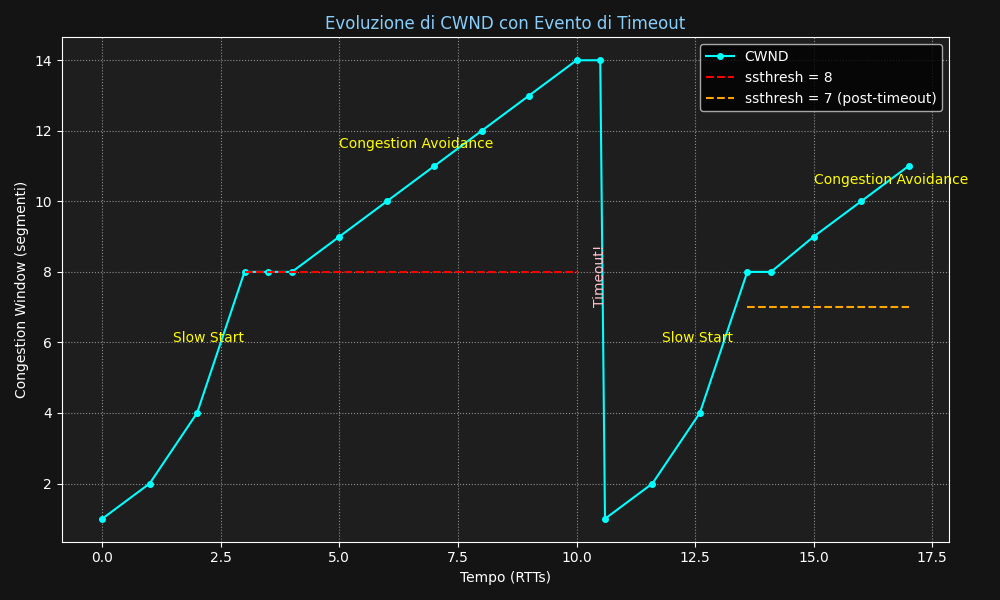
\includegraphics[width=0.8\textwidth]{images/cwnd_timeout.png}
    \caption{Effetto di un Timeout su CWND (Slow Start, Congestion Avoidance, Timeout, di nuovo Slow Start e Congestion Avoidance).}
    \label{fig:cwnd_timeout}
\end{figure}

\begin{figure}[H]
    \centering
    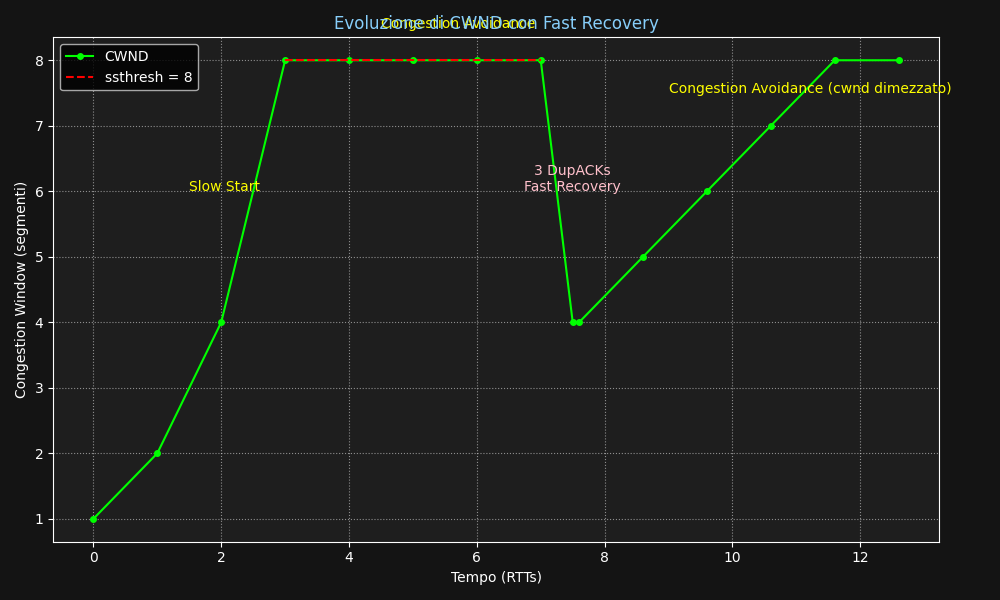
\includegraphics[width=0.8\textwidth]{images/cwnd_fastrecovery.png}
    \caption{Effetto di Fast Recovery su CWND (CWND si dimezza e continua in Congestion Avoidance).}
    \label{fig:cwnd_fastrecovery}
\end{figure}


\subsection{Sfide di TCP su MANET}
\begin{itemize}
    \item \textbf{Perdita di Pacchetti non dovuta a Congestione:} Errori wireless, collisioni, \textbf{rottura di rotte per mobilità}. TCP reagisce riducendo \texttt{cwnd} inutilmente.
    \item \textbf{Variazioni dell'RTT:} Cambi di rotta rendono difficile calcolare RTO accurato.
    \item \textbf{Out-of-Order Delivery:} Causa DupACKs e Fast Retransmit inutili.
    \item \textbf{Impatto Cache Obsolete (es. DSR):} Perdite su rotte obsolete, TCP reagisce male, lento recupero.
\end{itemize}
Molti lavori cercano di adattare TCP per MANET.

\section*{Possibili Argomenti per Seminario Finale (Generali)}
\begin{itemize}
    \item Multiple access techniques (including the impact of multiple antennas)
    \item Cellular system design
    \item Ad-hoc wireless networking
    \item Multiuser information theory
    \item Capacity of ad hoc networks
    \item Access techniques in wireless networks
    \item Dynamic resource allocation in wireless networks
    \item Cross layer design in wireless networks
    \item Adaptive modulation/coding in multiuser systems
    \item Power control in wireless networks
    \item Space-time processing for mobile communications
    \item MIMO techniques for multiuser systems
    \item Multiuser multicarrier /OFDM systems
    \item CDMA systems
    \item Interference cancellation / multiuser detection in CDMA
    \item Coding/spreading tradeoffs in CDMA
    \item CDMA vs. OFDM
    \item User location strategies in WiNet
    \item Multirate/multimedia over wireless networks
\end{itemize}

\section*{Possibili Argomenti per Seminario Finale}
\begin{itemize}
    \item Smart antennas
    \item Traffic models for multimedia data
    \item Energy efficient protocols for ad hoc and sensor systems
    \item Routing for ad hoc wireless networks
    \item Routing for vehicular wireless networks
    \item Performance of TCP/IP and/or ATM over wireless channels
    \item Performance of TCP/IP over multihop wireless networks
    \item Software radios
    \item Multiuser ultra wide band (UWB) systems
    \item HW constraints in wireless systems
    \item Wireless system services and killer applications
    \item Innovative and visionary wireless-enabled services
    \item RFID technologies
    \item Wireless frameworks' implementations
    \item Service frameworks for wireless devices synchronization
    \item Mobile IP
    \item Security issues in wireless systems
    \item Vehicular Network Technologies
    \item Wireless Monitoring
    \item IEEE 802.[11-22] and related special task groups
\end{itemize}

\end{document}